\documentclass[a4paper, 12pt]{article}
%\documentclass{book}

% Important Packages:
 \usepackage{amsmath}    % need for subequations
 \usepackage{amsfonts}
 \usepackage{amsthm}
 \usepackage{graphicx}   % need for figures
 \usepackage{verbatim}   % useful for program listings
 %\usepackage{subfig}  % use for side-by-side figures
 %\usepackage{wrapfig}
 %\usepackage{listings}	 % creates code blocks
 %\usepackage[colorlinks=true]{hyperref}   % use for hypertext links, including
                     % those to external documents and URLs
 %\usepackage{multirow}
 %\usepackage{tikz}
 %\usepackage{enumerate}
 %\usetikzlibrary{decorations.pathreplacing,decorations.pathmorphing}
 %\usetikzlibrary{calc}
 %\usepackage[colorinlistoftodos]{todonotes}
 \usepackage{tikz,tkz-euclide}
 
 \usetikzlibrary{calc,patterns,angles,quotes}
% \usetkzobj{all}

\def\deg{^{\circ}}
\newcommand\heading[1]{\ \\\large{\textbf{#1}}}
\newcommand\ora[1]{\overrightarrow{#1}}

\def\thm{Th\textsuperscript{\underline{m}}}

\newtheorem*{lemma}{Lemma}

%------------------end---preamble--------------------
 
 % Useful macros 
 \def\tcb#1{\color{blue}{#1}}
 \def\tcr#1{\color{red}{#1}}	
 \def\tcg#1{\color{green}{#1}}
 \def\be{\begin{eqnarray}}	 	\def\ee{\end{eqnarray}}
 \def\bea{\begin{eqnarray}}	 	\def\eea{\end{eqnarray}}
 \def\bean{\begin{eqnarray*}}	\def\eean{\end{eqnarray*}}
 
 \def\D{\displaystyle}
 \def\T{\textstyle}
 \def\l{\left}
 \def\r{\right}
 \def\nf{n_{\!f}} % quark flavours
 \def\pa{\partial}
 \def\eg{e.\,g.}
 \def\ie{i.\,e.}

 \def\be{\begin{equation}}
 \def\ee{\end{equation}}
 \def\bea{\begin{eqnarray}}
 \def\eea{\end{eqnarray}}
 \def\bean{\begin{eqnarray*}}
 \def\eean{\end{eqnarray*}}
 \def\gsim{\mathrel{\rlap{\lower0.2em\hbox{$\sim$}}\raise0.2em\hbox{$>$}}}
 \def\ksim{\mathrel{\rlap{\lower0.2em\hbox{$\sim$}}\raise0.2em\hbox{$<$}}}
 \def\kg{\mathrel{\rlap{\lower0.25em\hbox{$>$}}\raise0.25em\hbox{$<$}}}
 
 \def\AA{${\buildrel_{\circ} \over {\mathrm{A}}}$}
 \def\bm#1{\mbox{\boldmath$#1$}}
 \newcommand{\eq}[1]{(\ref{#1})} 
 \def\pd{\partial}
 \def\d{\textrm{d}} 
 \def\T{\textstyle}
 \def\eg{e.\,g.}	% exempli gratia (for the sake of example)
 \def\ie{i.\,e.}	% id est (that is)


 % Page configuration:
 \topmargin -2.0cm
 \oddsidemargin -0.85cm
 \evensidemargin -0.85cm
 \textwidth 18cm
 \textheight 24cm
 
\begin{document}
\begin{center}
\textbf{Stellenbosch Camp December 2018 \\ Senior Test 5} \\
\textbf{Solutions}
\end{center}
\vspace{5mm}

\begin{enumerate}
    
\item[1.]  \textit{Determine the number of ways to choose five numbers from the first eighteen positive integers such that any two chosen numbers differ by at least $2$.}

\begin{lemma}[`Stars and Bars'']
The number of ways of writing $n$ as a sum of $m$ non-negative natural numbers (where the order matters) is
\[
	\binom{n + m - 1}{m - 1}
\]
\end{lemma}
\begin{proof}
Consider a string of $n$ stars. We place $m - 1$ bars between the stars to divide them into $m$ groups. There is a bijection from the number of ways of placing the bars between the stars, and the number of ways of writing $n$ as a sum of $m$ non-negative integers: each groups represents one of the addends. The result follows by noting that we have $n + m - 1$ symbols in total, and must choose which $m - 1$ of them are bars.
\end{proof}

Let the five numbers be $x_1, x_2, \dots, x_5$, and let $x_0 = 1$ and $x_6 = 18$. Consider the differences $y_1 = x_1 - x_0, y_2 = x_2 - x_1, \dots, y_6 = x_6 - x_5$. Note that these differences uniquely determine the five chosen numbers, and that the sum of these differences is $x_6 - x_0 = 17$. Note also that the numbers $y_1, y_2 - 2, y_3 - 2, y_4 - 2, y_5 - 2, y_6$ are non-negative and sum to $17 - 4 \times 2 = 9$.

We thus wish to count the number of ways of writing $9$ as a sum of $6$ non-negative integers. By the lemma, this is given by
\[
	\binom{9 + 6 - 1}{6 - 1} = \binom{14}{5}.
\]

\qed


\vspace{5mm}
\item[2.]  \textit{Show that there exists an infinite arithmetic progression of natural numbers such that the first term is $16$ and the number of positive divisors of each term is divisible by $5$. Of all such sequences, find the one with the smallest possible positive common difference.}

Note that the sequence given by $a_n = 16(2n - 1)$ is an arithmetic progression with constant difference $32$. Since $2n - 1$ is odd, the largest power of $2$ which divides $a_n$ is $16$. We recall that if
\[
	n = {p_1}^{a_1} {p_2}^{a_2} \cdots {p_k}^{a_k}
\]
then the number of divisors of $n$ is given by $(a_1 + 1)(a_2 + 2) \cdots (a_k + 1)$. It follows that the number of divisors of $a_n$ is divisible by $(4 + 1) = 5$.

To see that this sequence has the smallest possible positive common difference, consider the second term of the sequence. Its number of divisors is divisible by $5$, so the exponent of one of the primes in its prime factorisation is at least $4$. (Note that $5$ is a prime, so $(a_1 + 1)$ must be divisible by $5$ for one of the exponents $a_i$.) If this prime factor is at least $3$, then the second term is at least $3^4 = 81$ which is larger than $a_2 = 48$. We see that the prime with exponent at least $4$ must be $2$, and so the second term is divisible by $16$. If it is not a power of $2$, then it must be at least $16 \times 3 = 48 = a_2$, so any sequence with a smaller common difference must have a second term which is a power of $2$. But the number of its divisors must be a multiple of $5$, so the exponent is at least $10 - 1$, and $2^9 > 48$.

\qed


\vspace{5mm}
\item[3.]  \textit{Suppose that Romeo and Juliet each have a regular tetrahedron, to the vertices of which some positive real numbers are assigned. They associate, to each edge of their tetrahedra, the product of the two numbers assigned to its end points. Then they write on each face of their tetrahedra the sum of the three numbers associated to its three edges. The four numbers written on the faces of Romeo’s tetrahedron turn out to coincide with the four numbers written on Juliet’s tetrahedron. Does it follow that the four numbers assigned to the vertices of Romeo’s tetrahedron are identical to the four numbers assigned to the vertices of Juliet’s tetrahedron?}

\textbf{Answer:} yes.

Let us prove that this conclusion can in fact be drawn. For this purpose we denote the numbers assigned to the vertices of Romeo's tetrahedron by $r_1, r_2, r_3, r_4$ and the numbers assigned to the vertices of Juliet's tetrahedron by $j_1, j_2, j_3, j_4$i in such a way that
\begin{eqnarray}
	r_2 r_3 + r_3 r_4 + r_4 r_2 = j_2 j_3 + j_3 j_4 + j_4 j_2 \\
	r_1 r_3 + r_3 r_4 + r_4 r_1 = j_1 j_3 + j_3 j_4 + j_4 j_1 \\
	r_1 r_2 + r_2 r_4 + r_4 r_1 = j_1 j_2 + j_2 j_4 + j_4 j_1 \\
	r_1 r_2 + r_2 r_3 + r_3 r_1 = j_1 j_2 + j_2 j_3 + j_3 j_1
\end{eqnarray}

We intend to show that $r_1 = j_1$, $r_2 = j_2$, $r_3 = j_3$, and $r_4 = j_4$, which clearly suffices to prove our claim. Now let
\[
	R = \{ i | r_i > j_i \}
\]
denote the set of indices where Romeo's corresponding number is larger, and define similarly
\[
	J = \{ i | r_i < j_i \}.
\]

If we had $|R| > 2$, then w.l.o.g. $\{1, 2, 3\} \subseteq R$, which easily contradicts $(4)$. Therefore $|R| \leq 2$, so let us suppose for the moment that $|R| = 2$. Then w.l.o.g. $R = \{1, 2\}$, \ie $r_1 > j_1$, $r_2 > j_2$, $r_3 \leq j_3$, $r_4 \leq j_4$. It follows that $r_1 r_2 - r_3 r_4 > j_1 j_2 - j_3 j_4$, but $(1) + (2) + (3) - (4)$ actually tells us that both sides of this strict inequality are equal.

This contradiction yields $|R| \leq 1$ and, replacing the roles of Romeo and Juliet played in the argument just performed, we similarly infer $|J| \leq 1$. For these reasons, at least two of the four desired equalities hold, say $r_1 = j_1$ and $r_2 = j_2$. Now using $(3)$ and $(4)$, we easily get $r_3 = j_3$ and $r_4 = j_4$ as well.
\qed
\vspace{6mm}

\item[4.]  \textit{Determine all pairs $(a,b)$ of integers with the property that the numbers $a^2+4b$ and $b^2+4a$ are both perfect squares.}

 If either $a$ or $b$ is 0, then both must be perfect squares. If $a = b$, then we must solve $a^2 + 4a = k^2$ where $k \in \mathbb{Z}$. This gives us $(a+2-k)(a+2+k) = 4$ which can easily be solved to give the solution $a = b = -4$. If $a = -b$, then we similarly obtain $(a-2-k)(a-2+k) = 4$ which yields no solutions. \\

We can now assume $|a| > |b| \geq 1$.  If $|a| > 4$, we have
\begin{equation*}
    (|a| - 4)^2 = a^2 - 8|a| + 16 \leq a^2 - 4|a| \leq a^2 + 4b \leq a^2 + 4|a| < (|a| + 2)^2
\end{equation*}
This bounds $a^2 + 4b$ between two squares. Furthermore, noting that $a^2 + 4b$ and $b^2 + 4a$ have the same pairty, we thus have that either $a^2 + 4b = a^2$ or $a^2 + 4b = (|a| - 2)^2$. The former case yields $b = 0$ which has been covered, thus we assume $a^2 + 4b = (|a| - 2)^2$, which implies $b = 1 - |a|$.

Therefore, $b^2 + 4a = a^2 - 2|a| + 1 + 4a$ is a perfect square. We consider two cases:

\textbf{Case 1}: $a > 0$. Thus $b^2 + 4a = a^2 + 2a + 1 = (a+1)^2$ which is a square.

\textbf{Case 2}: $a < 0$. Thus $b^2 + 4a = a^2 + 6a + 1 = (a + 3)^2 - 8$. Now, the only case which will give two squares a difference of 8 apart is $1, 9$, which yields $a = -6$ and $b = -5$.

Finally, we consider the cases where $|a| \leq 4$. This only yields the solution $(-4, -4)$. We thus conclude the solutions are
\begin{align*}
    a = 0 &\textrm{ and } b = k^2, \quad k \geq 0 \\
    \textrm{ or } \quad a = k^2 &\textrm{ and } b = 0, \quad k \geq 0 \\
    \textrm{ or } \quad \hspace{1.5mm} a = k &\textrm{ and } b = 1-k, \quad k \in \mathbb{Z} \\
    \textrm{ or } \quad \hspace{2.5mm} (a, b) &\in \{(-4, -4), (-5, -6), (-6, -5) \}
\end{align*}

\qed


\vspace{5mm}

% USAMO 1999 (official solution modified for 2018)
\item[5.]   \textit{Two players play a game on a line of 2018 squares. Each player in turn puts either S or O into an empty square. The game stops when three adjacent squares contain S, O, S in that order and the last player wins. If all the squares are filled without getting S, O, S, then the game is drawn. Show that the second player can always win.}

 Suppose a square is such that if you play there then that allows your opponent to win on the following move. If you play an O, then your opponent must win by playing an adjacent S. So we must have S 1 2 3, where 1 and 2 are empty and you play O on square 1. But you also lose if you play S, so your opponent must then win by playing O on 2, which means that 3 must already contain an S. But now the situation is symmetrical, so that 2 is also a losing square. Thus, until someone plays on one of them, losing squares always occur in pairs.

The board has an even number of squares, so the first player always faces a board with an even number of squares not yet occupied, whereas the second player always faces a board with an odd number of squares not yet occupied. Thus provided (1) there is at least one pair of losing squares, (2) he never plays on a losing square, and (3) he makes the obvious winning move if the first player ever creates the opportunity, then the second player is sure to win, because the first player will eventually face a board with only losing squares available for play. \\

To make sure there is at least one pair of losing squares the second player must create it. He can always do this by placing an S on his first move well away from the first player's move and from the edges of the board. Then on his second move (assuming the first player has not been stupid enough to allow him an immediate win) he can always play another S three away from it, creating a pair of losing squares. Thereafter, he must simply take care to win if there is a winning move and otherwise to avoid losing plays.

\qed



\item[6.]  \textit{Isosceles $\triangle ABC\ (AC=BC)$ is inscribed in a circle $k$. A point $M$ lies on the side $BC$. A point $N$ from the ray $AM$ ($M$ lies between $A$ and $N$) is such that $AN=AC$. The circumcircle of $\triangle MCN$ intersects $k$ at $C$ and $P$, where $P$ is from the arc $BC$ not containing $A$. The lines $AB$ and $CP$ intersect at $Q$. Prove that $\angle QMB = \angle QMN$.}


	Denote $\angle MAC=\alpha$ and $\angle ACB=\beta$. Let $J$ the incentre of $\triangle AMC$.
	
	    \vspace{10mm}
		\begin{figure}[h]
		\begin{center}
		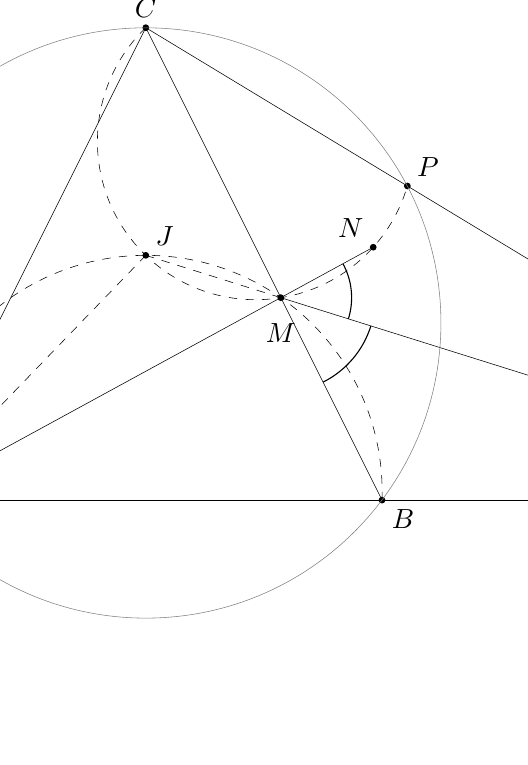
\begin{tikzpicture}[scale=3]
			\useasboundingbox (-.5,-1) rectangle  (1.5,2);
			\tkzDefPoint(-1,0){A}
			\tkzDefPoint(1,0){B}
			\tkzDefPoint(0,2){C}
			\tkzDefCircle[circum](A,B,C)\tkzGetPoint{O}
			\tkzDefBarycentricPoint(C=3,B=4)\tkzGetPoint{M}
			\tkzInterLC(A,M)(A,C)\tkzGetSecondPoint{N}
			\tkzDefCircle[circum](M,N,C)\tkzGetPoint{I}
			\tkzInterCC(I,C)(O,C)\tkzGetFirstPoint{P}
			\tkzInterLL(C,P)(A,B)\tkzGetPoint{Q}
			\tkzDefCircle[in](A,M,C)\tkzGetPoint{J}

			\tkzDrawPoints[fill=black](A,B,C,M,N,P,Q,J)
			\tkzDrawSegments(A,Q B,C C,A A,N C,Q M,Q)
			\tkzDrawSegments[dashed](A,J J,M)
			\tkzMarkAngle[size=0.3](Q,M,N)
			\tkzMarkAngle[size=0.4](B,M,Q)

			\tkzDrawArc[rotate,dashed,color=black](I,C)(210)
			\tkzDefCircle[circum](A,B,M)\tkzGetPoint{K}\tkzGetLength{r}
			\tkzDrawArc[rotate,dashed,color=black](K,B)(185)
			\tkzDrawCircle(O,A)
			\tkzLabelPoints[above](C)
			\tkzLabelPoints[below=0.2](M)
			\tkzLabelPoints[below left](A,Q)
			\tkzLabelPoints[below right](B)
			\tkzLabelPoints[above right](J,P)
			\tkzLabelPoints[above left](N)
			
			\end{tikzpicture}
		\end{center}		
		\end{figure}
		\vspace{-5mm}
		
	 It follows that $\angle AJM=90\deg+\beta/2$ and $\angle ABM=90\deg- \beta/2$, which implies that the quadrilateral $ABMJ$ is inscribed in a circle $k_1$. Analogously we have that the quadrilateral $MNCJ$ is inscribed in a circle $k_2$ which is just the circumcircle of $\triangle MCN$. Therefore $P$ is a point on $k_2$. Since $QA \cdot QB =QC \cdot QP$ we conclude that $Q$ lies on $JM$, which is the angle bisector of $\angle BNC$. Thus $\angle QMB = \angle QMN$
	



\qed





    

\end{enumerate}
\end{document}




